\documentclass{sig-alternate}

% UTF8 support
\usepackage[utf8x]{inputenc}


\usepackage{hyperref}
\usepackage{epsf,graphicx}
\graphicspath{{figures/}}
\usepackage{subfigure}
%\usepackage[colorinlistoftodos]{todonotes}

\usepackage[usenames,dvipsnames]{xcolor}
\usepackage{tikz}
\usetikzlibrary{positioning, calc}


\newcommand{\eg}{{\textit{e.g.~}}}
\newcommand{\etal}{{\textit{et al.~}}}
\newcommand{\ie}{{\textit{i.e.~}}}

%
% --- Author Metadata here ---
\conferenceinfo{10th ACM/IEEE International Conference on Human-Robot Interaction}{2015 Portland, USA}
%\CopyrightYear{2007} % Allows default copyright year (20XX) to be over-ridden - IF NEED BE.
%\crdata{0-12345-67-8/90/01}  % Allows default copyright data (0-89791-88-6/97/05) to be over-ridden - IF NEED BE.
% --- End of Author Metadata ---

\title{\LARGE \bf
Children Teach a Robot to Write: A Teachable Robotic Agent which Engages in Simulated Handwriting %still not sure
% what about:
% When Children Teach a Robot to Write
% ?
}

\numberofauthors{1} 
%\author{
%\alignauthor
%Deanna Hood, Séverin Lemaignan, Pierre Dillenbourg\\
%   \affaddr{Computer-Human Interaction in Learning and Instruction Laboratory (CHILI)}\\
%   \affaddr{École Polytechnique Fédérale\\ de Lausanne (EPFL)}\\
%   %\affaddr{CH-1015 Lausanne, Switzerland}\\
%   \email{firstname.lastname@epfl.ch}
%}

%(DH) my EPFL email address won't work for much longer....


\begin{document}



\maketitle

%%%%%%%%%%%%%%%%%%%%%%%%%%%%%%%%%%%%%%%%%%%%%%%%%%%%%%%%%%%%%%%%%%%%%%%%%%%%%%%%
\begin{abstract}

This article presents a novel robotic partner which children can teach
handwriting.  The system relies on the \emph{learning by teaching} paradigm to
build an interaction, so as to stimulate meta-cognition, empathy and
increased self-esteem in the child user.  We hypothesise that use of a
humanoid robot in such a system could not just engage an unmotivated student,
but could also present the opportunity for children to experience
physically-induced benefits encountered during human-led handwriting
interventions, such as motor mimicry.

By leveraging simulated handwriting on a synchronised tablet display, a {\sc
nao} humanoid robot with limited fine motor capabilities has been configured as
a suitably embodied handwriting partner. Statistical shape models derived from
principal component analysis of a dataset of adult-written letter trajectories
allow the robot to draw purposefully deformed letters. By incorporating feedback
from user demonstrations, the system is then able to learn the optimal
parameters for the appropriate shape models. 

Preliminary in situ studies have been conducted with primary school classes to
obtain insight into children's use of the novel system.  Children aged 6-8
successfully engaged with the robot and improved its writing to a level which
they were satisfied with. The validation of the interaction represents a
significant step towards an innovative use for robotics which addresses a
widespread and socially meaningful challenge in education. 

\end{abstract}


%%%%%%%%%%%%%%%%%%%%%%%%%%%%%%%%%%%%%%%%%%%%%%%%%%%%%%%%%%%%%%%%%%%%%%%%%%%%%%%%
\section{INTRODUCTION}

Handwriting difficulties in children at an early age often negatively affect
the academic performance of the students \cite{Christensen2005}, in addition to
their self-esteem being adversely affected \cite{Malloy1995}, causing them to
shy away from expressing what they know \cite{Medwell2008}.
Successful interventions for children with handwriting difficulties involve the
student in many sessions where they are engaged in physically practising the
skill \cite{Hoy2011}. However, the link between handwriting difficulties and low
self-efficacy \cite{Engel-Yeger2009} results in children who are unmotivated to
participate in such sessions, potentially leading to a developmental arrest in
the acquisition of the skill. 

The \emph{learning by teaching} paradigm, which engages the target student in
the act of teaching another, has been shown to produce motivational,
meta-cognitive, and educational benefits in a range of disciplines
\cite{Rohrbeck2003}. To our best knowledge, the application of the paradigm to
handwriting intervention remains, however, unexplored. One reason for this may due
to the requirement of an appropriately unskilled peer for the target child to
tutor, as this may present a logistical constraint if the target child is the
lowest performer in their class.  In some cases, it may be appropriate for a
peer or teacher to simulate a na\"ive learner for the target child to teach.
For handwriting, where one's skill level is visually evident, however, this
acting is likely to be eventually detected. As such, there is motivation for the
use of a teachable agent which can be configured for a variety of skill levels,
and for which children do not have preconceptions about its handwriting ability.

We present the development of a novel teachable agent
that intentionally makes mistakes typical of children learning
handwriting. Through this capability, the robot can be taught by
children, who themselves may learn through their teaching.

Teachable computer-based agents have previously been used to encourage the 
``protégé effect'', wherein students invest more effort into learning when it
is for a teachable agent than for themselves~\cite{Chase2009}. As we are 
concerned with learning of a physical skill, the learning agent developed is 
embodied in a humanoid robot which is capable of physically demonstrating 
handwriting trajectories to its child learning partner.
This is supported by the potential for motor mimicry to yield significant 
improvements in handwriting interventions in which letter formations are 
demonstrated to participants~\cite{Berninger1997}.

Werfel suggests in~\cite{Werfel2014} that, until now, most of the work investigating how
humans can teach robots (in particular, physical skills) focuses on the robot's
benefits, and not so much on the learning experienced by the human tutor. Our
work focuses on this latter aspect. A robotic learning agent which employs the learning by teaching paradigm has 
previously been developed by Tanaka and Matsuzoe~\cite{Tanaka2012}. In their
system, children learn vocabulary by teaching the {\sc nao} robot to act out 
verbs. The robot is tele-operated and mimics the actions that the children
teach it, but with no long-term memory or learning algorithm in place.

Our work significantly extends this line of work in two directions, first by
proposing an autonomous robotic partner, second by investigating the context
of children's acquisition of a challenging physical skill (handwriting).

Due to the intended use in a school environment, a commercially
affordable {\sc nao} humanoid robot has been used. Its writing capabilities 
have been implemented by leveraging synchronisation with a tablet display to
simulate fine motor skills otherwise infeasible for the robot. 

Within this article, Section \ref{sec:learningAlgorithm} presents the novel work in the area of
artificial intelligence to develop a learning algorithm suitable for a teachable
agent in the context of handwriting. Section \ref{sec:robotWriting} details the
extension of this algorithm to an embodied robotic learning agent, including the
new approach for achieving simulated fine motor skills on commercially
affordable humanoid robots. Section \ref{sec:experiment} explores the 
contributions made to the study of human-robot interaction, in discussing the
use of the system with primary school children and its potential as a tool for
addressing wider pedagogical research questions in education. Finally, Section \ref{sec:futureWork} addresses the challenges which are faced in extending this system to a level suitable for long-term studies, and Section \ref{sec:conclusions} concludes by reiterating the content and impact of the article's contributions.



%%%%%%%%%%%%%%%%%%%%%%%%%%%%%%%%%%%%%%%%%%%%%%%%%%%%%%%%%%%%%%%%%%%%%%%%%%%%%%%%
\section{A Learning Agent in the Context of Handwriting} \label{sec:learningAlgorithm}

A parameterisation of letters and their deformities was sought such 
that different quality shapes can be generated, depending on the parameters input to
the letter models. This allows us to configure the system such as to improve its writing 
by modifying the parameters based on feedback from the 
reinforcement learning partner (Section~\ref{sec:learningAlg}). 


\subsection{Shape Modelling of Letters} \label{sec:writingGeneration}

We use statistical shape modelling as an approach for a shape model which can
appropriately represent realistic variations in shapes. Statistical shape
modelling is an application of principle component analysis (PCA), where a
linear transform which de-correlates data vectors is found~\cite{Stegmann2002}
and allows for dimensionality reduction. 

PCA is performed on a set of letter paths captured from a digital pen,
using the UJI Pen Characters 2 dataset \cite{Llorens2008} with 120 instances of
each letter (2 repetitions from 60 adult users). While it may be appropriate in future work to
identify the location of salient features of the shapes which are robust to 
unanticipated user input (such as shapes drawn backwards),
the features are currently taken as $n$ uniformly spaced points along the shape
path. The
points are arranged into an observation vector presented in (\ref{eq:obsVec}),
where $x_i$ and $y_i$ represent the coordinates of each of the points along the
path. The observation shapes are normalised to have a unit maximum dimension 
and centre at the origin.

\begin{equation}\label{eq:obsVec}
{\bf x} = [x_1, x_2, \ldots, x_n, y_1, y_2, \ldots, y_n]^T
\end{equation}

Equation (\ref{eq:projection}) represents the projection from the original 
$2n$-dimensional feature space $(n=70)$ to a reduced $N$-dimensional space, where ${\bf p}$
contains the coordinates in the $N$-dimensional space with ${\bf 0}$-origin,
calculated as in (\ref{eq:paramCalc}). 
${\bf \Phi }$ is
an orthogonal $2n\times N$ matrix composed of the eigenvectors ${\bf v}_i$ corresponding to
the largest $N$ eigenvalues ($\lambda_i$) of the covariance matrix of the
observations, as shown in (\ref{eq:transformCalc}) \cite{Stegmann2002}. 
If there is correlation between the points in the observations, there will be
eigenvalues of the covariance matrix which are close to zero. As such, removing
the associated eigenvectors from ${\bf \Phi}$ allows for dimensionality
reduction with minimal impact.


\begin{equation}\label{eq:projection}
{\bf \tilde{x}=\bar{x}+\Phi p}
\end{equation}
\begin{equation}\label{eq:paramCalc}
{\bf p} ={\bf \Phi}^T ({\bf {x}-\bar{x}})
\end{equation}
\begin{equation}\label{eq:transformCalc}
{\bf \Phi} = [{\bf v}_1, {\bf v}_2, \ldots, {\bf v}_N]^T
\end{equation}

PCA is performed on all of the paths of a particular allograph in the
dataset individually, to reduce the $2n$-dimensional space for that shape to one 
with $N=10$ dimensions.
As such,
each shape may be approximated by the mean shape of the allograph plus a sum of the top 10
eigenvectors, weighted by the parameter vector ${\bf p}$. 
%Indeed, the amount of variance in the dataset
%that is explained by each eigenvector ${\bf v}_i$ is $\sqrt{\lambda_i}$, and
%therefore the proportion of the variance explained by each dimension/eigenvector
%is as shown in (\ref{eq:proportionVar}).
%
%\begin{equation}\label{eq:proportionVar}
%\%var_i = \frac{\sqrt{\lambda_i}}{\sum_{i=1}^{N}\sqrt{\lambda_i}}\times 100\%
%\end{equation}

(\ref{eq:projection}) may also be used
to generate new shapes based on the parameters ${\bf p}$ which are used. ${\bf
p}={\bf 0}$ will yield the mean shape, and variations to each of the $N$ values
in ${\bf p}$ will cause a change in the shape represented by the corresponding
eigenvector (Figure \ref{fig:deviations_sPrint}). 
For the dataset presented in Figure \ref{fig:deviations_sPrint}, the
eigenvectors associated with the 3 largest eigenvalues explain 78.5\% of the
variance in the dataset, illustrating the capability of the statistical shape
modelling approach to produce compact parameterisation of shapes. 

%Clusters within paths of a particular letter have been identified using K-means
%clustering to group different styles of writing the letter (\emph{allographs}),
%such that the parameters in the resulting model are only representative of the
%specific allograph of the letter in the dataset. 
% * <deanna.m.hood@gmail.com> 2014-09-03T13:05:23.576Z:
%
% in the end this was pointless so maybe not worth mentioning
%

\begin{figure}[thpb]
\centering
\subfigure{
\raisebox{-0.5\height}{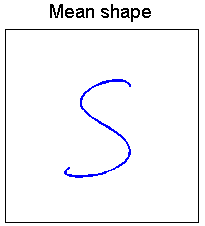
\includegraphics[width=0.05\textwidth]{figures/sPrint_mean.png}
}}
\subfigure{
\raisebox{-0.5\height}{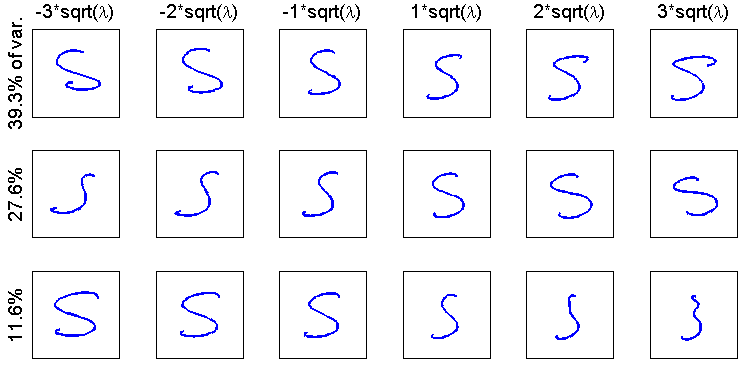
\includegraphics[width=0.35\textwidth]{figures/sPrint_top3.png}
}}
\caption[The mean shape and the effect of varying the first three parameters of
the shape model derived from PCA from the dataset of print `s'
shapes.]{\label{fig:deviations_sPrint}The mean shape (left) and the effect
    (right) of varying the first three parameters (each row) of a shape model.
     The extent to which each
parameter is varied is dependent on the eigenvalue $\lambda$ corresponding to
the parameter's eigenvector. The percentage of the total variance in the dataset
explained by each parameter is shown to the left of the corresponding row. }

\end{figure}



Interestingly, although the parameters are the result of an \emph{unsupervised} 
shape analysis, they still represent variations which could have
been intuitively identified by a manual parameterisation. For example, for the
model shown in Figure \ref{fig:deviations_sPrint}, the parameters may represent
the height of the top half of the letter compared to the bottom half, the width
of the overall shape, etc. The ability to generate varied levels of deformations
which may be ascribed descriptive interpretations (not just numerical) is an
advantage of this method, given its intended use with humans. It is, for instance,
possible for a teacher to create initial letters with a particular feature (a wide
`s' or a `d' with a large loop, for example).


\subsection{Generating Poor Letters}

As explained, new letters can be generated by varying the parameter values 
for a shape model in accordance with (\ref{eq:projection}). By choosing
parameter values which lie within the observed range in the dataset, it is
possible to produce letters which are more likely to be reasonable looking.
When the parameter values are outside of the range observed in the dataset, they
are less likely to represent shapes from the dataset of adult-written letters, 
and as a result are more likely to represent poor shapes.
Figure \ref{fig:sampleLetters} illustrates sample letters generated from the
models of `e' and `g' by selecting random values for the first 5 parameters 
from a distribution with
standard deviation of $3\sqrt\lambda_i$ rather than the $\sqrt\lambda_i$
standard deviation observed in the dataset.

\begin{figure}[thpb]
\centering
\subfigure{\raisebox{-0.5\height}{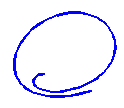
\includegraphics[height=0.04\textwidth]{figures/e1.png}}}
\subfigure{\raisebox{-0.5\height}{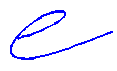
\includegraphics[height=0.025\textwidth]{figures/e4.png}}}
\subfigure{\raisebox{-0.5\height}{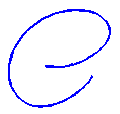
\includegraphics[height=0.04\textwidth]{figures/e3.png}}}
\subfigure{\raisebox{-0.5\height}{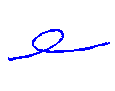
\includegraphics[height=0.04\textwidth]{figures/e5.png}}}~~~~~
\subfigure{\raisebox{-0.5\height}{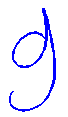
\includegraphics[height=0.06\textwidth]{figures/g1.png}}}
\subfigure{\raisebox{-0.5\height}{
\includegraphics[height=0.06\textwidth]{figures/g3.png}}}
\subfigure{\raisebox{-0.5\height}{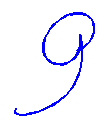
\includegraphics[height=0.06\textwidth]{figures/g4.png}}}
\subfigure{\raisebox{-0.5\height}{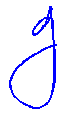
\includegraphics[height=0.06\textwidth]{figures/g5.png}}}
\caption[Sample letters generated from the PCA shape model on `e' and `g'
paths.]{\label{fig:sampleLetters}Sample letters generated from the PCA shape
model on `e' (left) and `g' paths (right), generated randomly from
parameters with $3\times$ the standard deviation observed in the dataset.}

\end{figure}

In~\cite{Chandra2013}, Chandra found that children aged 4-6 years participating
in a handwriting peer tutoring pilot study most often made mistakes
qualitatively classified as inappropriate \emph{internal proportions} or
\emph{global deformations}. As exemplified in Figure \ref{fig:sampleLetters},
the shapes generated by the system exhibit the same kind of deformities. Chandra
identifies other, less common, mistakes that involve topological changes (like
letters being broken in subparts, extra strokes, etc.). Using a database of
children's letters when available may yield potential for better parameterising
these other mistakes. However, as an initial approximation, the shape models
generated from PCA on a dataset of only adults' writing have shown to be
well-suited to generate `poor' letters that children were able to recognise and
successfully improve.


\subsection{Responding to Feedback}\label{sec:learningAlg}

In addition to generating letters by varying input parameters, the statistical 
shape model of Section \ref{sec:writingGeneration} may also be used 
to determine a particular letter's parameters, given the model. The parameters of user-drawn
letters may therefore be used in order implement a 
learning algorithm which adapts to the user's feedback via demonstration letters.

The statistical shape model is used to determine the parameters of a
demonstration shape by projecting the features of the observed shape into the
lower-dimensional space determined by the model. Mathematically, given a
demonstration ${\bf x}_{demo}$, the associated parameters may be determined as in
(\ref{eq:param}), which will reconstruct an approximate shape.

%really this is the same as eq 3
\begin{equation}\label{eq:param}
{\bf p}_{demo} ={\bf \Phi}^T ({\bf{x}_{demo}}-\bf{\bar{x}})
\end{equation}

%The parameters which are determined for a shape in (\ref{eq:param}) will not
%reconstruct the shape exactly if $N<2n$, but rather will reconstruct the closest
%point in the $N$-dimensional space which the eigenvectors span.

For the statistical shape model employed by the system, the method for
responding to user demonstrations is to move the learning algorithm's parameters
towards those of the demonstration. In the results presented in this work, the
linear update equation shown in (\ref{eq:update}) is used, where ${\bf p}$ is the
learned parameter vector at time step $k$, and $\alpha$ is the learning rate,
between 0 and 1.  

\begin{equation}\label{eq:update}
{\bf p}^{(k+1)} = {\bf p}^{(k)} + ({\bf p}_{demo}-{\bf
p}^{(k)})\times\alpha
\end{equation}

Figure \ref{fig:demonstrationShapes2} illustrates the response of the system to
demonstrations from a child for the letter `s' using a learning rate of
$\alpha=1/2$. Observe that even poorly-written demonstrations allow the system to improve.

\begin{figure}[thpb]
    \centering
    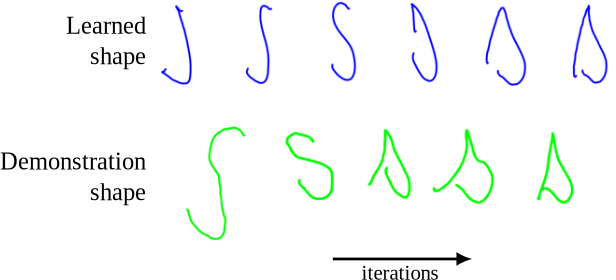
\includegraphics[width=0.45\textwidth]{figures/learningSdemo}
    \caption{\label{fig:demonstrationShapes2}Example of the learning algorithm
    responding (top) to user demonstration of shapes (bottom) for the letter `s' (demonstrations received from two 7-8 year-old children taking turns).}
\end{figure}

It is possible that parameters ${\bf p}^{(k)}$ and ${\bf p}_{demo}$, which
individually yield acceptable shapes, produce parameters ${\bf p}^{(k+1)}$
which yield an unacceptable shape. This is especially true if the demonstration
shape is of a different style to that learnt at time $k$, as there are no
restrictions imposed on parameter values. However, the proposed method for adapting to
the demonstration shapes has the advantage of being able to recover from such a situation: with further
demonstrations of the same letter, the system would eventually approach the
demonstration shape (see Figure \ref{fig:eDemo}. As a result, the event of poor-looking 
intermediate letters
would not limit the interaction later proposed in Section \ref{sec:experiment}
in a technical sense, but it may influence the user's \emph{perception} of the learning
agent. It remains to be seen if it is necessary to avoid such an event
mathematically.

\begin{figure}[thpb]
    \centering
    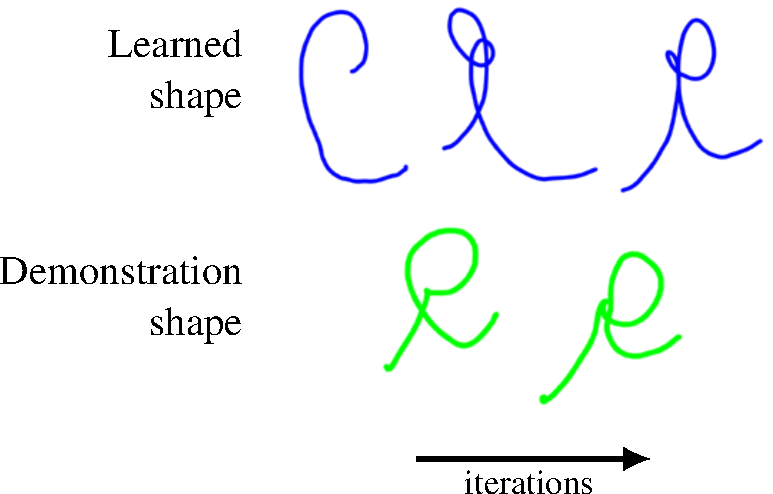
\includegraphics[width=0.3\textwidth]{figures/learningEdemo}
    \caption{\label{fig:eDemo}Example of the learning algorithm
    responding (top) to user demonstration of shapes (bottom) for the letter `e', passing through a parameter state which yields a poor letter (demonstrations received from a 7-8 year-old child).}
\end{figure}



%%%%%%%%%%%%%%%%%%%%%%%%%%%%%%%%%%%%%%%%%%%%%%%%%%%%%%%%%%%%%%%%%%%%%%%%%%%%%%%%
\section{An Embodied Handwriting Learning Agent with the NAO Humanoid Robot}
\label{sec:robotWriting}

In order to develop a teachable agent that is appropriate for engaging a child
in the learning by teaching paradigm, we have established capabilities for the robot 
to engage in handwriting and interactive turn-taking.

The {\sc nao} V4 humanoid robot, which has been developed by Aldebaran Robotics and 
purposely designed to look approachable \cite{Gouaillier2008}, is used for
this work. It is a commercially affordable biped robot, 58cm tall, with 25
degrees of freedom, two cameras, speech capabilities and the ability to
autonomously execute a range of tasks.

Precise control over what the robot is writing is necessary in the
proposed application of a handwriting. Because
of the limited fine motor skills possible with such an affordable robot, in
addition to the absence of force feedback and other technical necessities, we
have configured the {\sc nao} to use simulated handwriting with a synchronised tablet
to achieve this level of control. 

The development of the necessary components for embedding the handwriting learning
algorithm presented in Section \ref{sec:learningAlgorithm} in the humanoid agent
are presented in the sections which follow.

\subsection{Robot Trajectory Following Movements}

Using simulated handwriting provides an opportunity for the robot's writing to
appear smoother than would be achievable with a writing instrument. However, the
robot's motions must still sufficiently match the displayed trajectory in order
capture the engagement of the child participant in the action. Aldebaran's NaoQi API
is used for the inverse kinematics of the trajectory following. The Robot
Operating System (ROS)\footnote{The ROS stack for {\sc nao} is available at:
\url{http://wiki.ros.org/nao_robot}.} is used for integration of the {\sc nao}
with external reference frames, such as the tablet's location, 
using the $tf$ transformation library \cite{Foote2013}.

When using simulated handwriting, it is no longer necessary that the robot
engages in the typical style of handwriting of using a writing instrument at a desk.
Having the robot point at a vertical writing surface to cause the
trajectory to appear (as in Figure \ref{fig:naoWriting}) has several
advantages:

\begin{itemize}

    \item The working space of the robot increases, both in the technical sense
        and the interaction sense: someone can, in theory, show the tablet to
        the robot from across the room and have it still respond, without
        needing the tablet to be within arm's reach.

    \item Concerns about whether or not the child would start mimicking the
        robot's incorrect writing form (\eg pen grip) are mitigated. 

    \item Perhaps most significantly, the accuracy of the matching of the
        robot's motion with the trajectory displayed on the tablet is not as
        critical. This is because a pen tip would be expected to touch the
        tablet exactly at the trajectory point, while a fingertip may not.

\end{itemize}

\begin{figure}[thpb]
     \begin{center}
            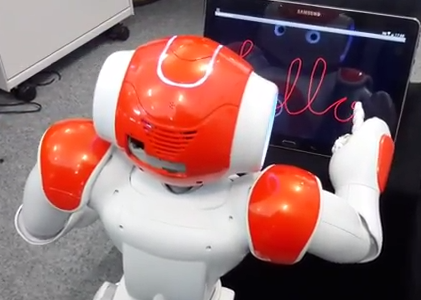
\includegraphics[width=0.7\linewidth]{figures/naoWriting2.png}
    \end{center}
    \caption{A demonstration of the robot simulating the writing of a word with
    its finger. The motion of the robot is synchronised with the display of the
    tablet, communicating over ROS.\protect\footnotemark}%

   \label{fig:naoWriting}
\end{figure}
%\footnotetext{See \url{https://www.youtube.com/watch?v=2qWFSJRxCU0} for a video of the synchronised 
\footnotetext{See \url{[anonymized]} for a video of the synchronised 
writing demonstration. }

We have therefore designed the system in such a way that the robot is
simulating handwriting by pointing at the tablet\footnote{Teachers interviewed
for their feedback on the system advised that children are asked to draw letters
in the air in a similar manner as part of their handwriting education. The behaviour 
is hence not unfamiliar to children.}. As
interacting with a tablet with one's finger is not uncommon, this may aid the
acceptance of the writing style by users. 

Because
motion planning is performed with respect to the hand of the robot, rather than
its fingertip, one or two of the orientation degrees of freedom of the hand
are fixed to keep the finger approximately perpendicular to the writing surface,
depending on the desired accuracy. The remaining free orientation(s), coupled
with the whole-body motion control available, allow for a sufficient working
space for writing on the entire tablet.

\subsection{Synchronisation with the Tablet Trajectory Display}\label{sec:tabletSynch}

%After getting the robot to trace writing trajectories, the next step towards
%simulated handwriting is getting the trajectories of the robot's `writing' to
%display on an Android tablet. 

To enable the robot's `writing' to display while the robot is tracing
trajectories, ROS is used for the communication between the devices,
including the Android tablet\footnote{For more information about ROS on Android
devices see \url{http://wiki.ros.org/android}}. As a result, aspects of the
networking between the tablet and the robot, such as the overheads associated
with connections, ports, message formats, etc. have been simplified. 

An Android application has been developed to receive the trajectory message over
a ROS topic and display the trajectory as an
animation. Synchronisation between the tablet and the robot is achieved by
using NTP servers to synchronise device clocks; passing only the necessary number of points (7)
to the robot's motion planner to improve timing accuracy; and not running 
computationally expensive tasks on the robot (such as camera publishing) while it 
is writing.

% \begin{itemize}

%     \item sending a requested start time accompanying the trajectory, which is
%         sufficiently in the future, to account for varying transmission delays
%         to the nodes on different devices,

%     \item synchronising all clocks with NTP servers such that the ROS time used
%         for responding to the requested start time is the same at all nodes,

%     \item reducing the number of points along the trajectory passed to the
%         robot's motion planner to improve timing accuracy, and

%     \item not running computationally expensive tasks on the robot (such as
%         camera publishing) while it is writing as this interferes with the
%         requested timings between points. 

% \end{itemize}

To instruct the robot where to write, the robot has been configured to detect a
particular fiducial marker, a \emph{chilitag}\footnote{See
\url{https://github.com/chili-epfl/ros_markers} for more information on the
fiducial markers used.}, with the camera located in its head, and to use that to
determine the relative position of the writing surface (Figure
\ref{fig:tabletDetection}). When used in an interaction involving a participant, this
allows a user to move the tablet as required for the interaction. The tablet is 
assumed to be stationary during the writing process as detecting the tablet interferes
with the robot's adherance to writing synchronisation.

\begin{figure}[htpb]
    \centering
    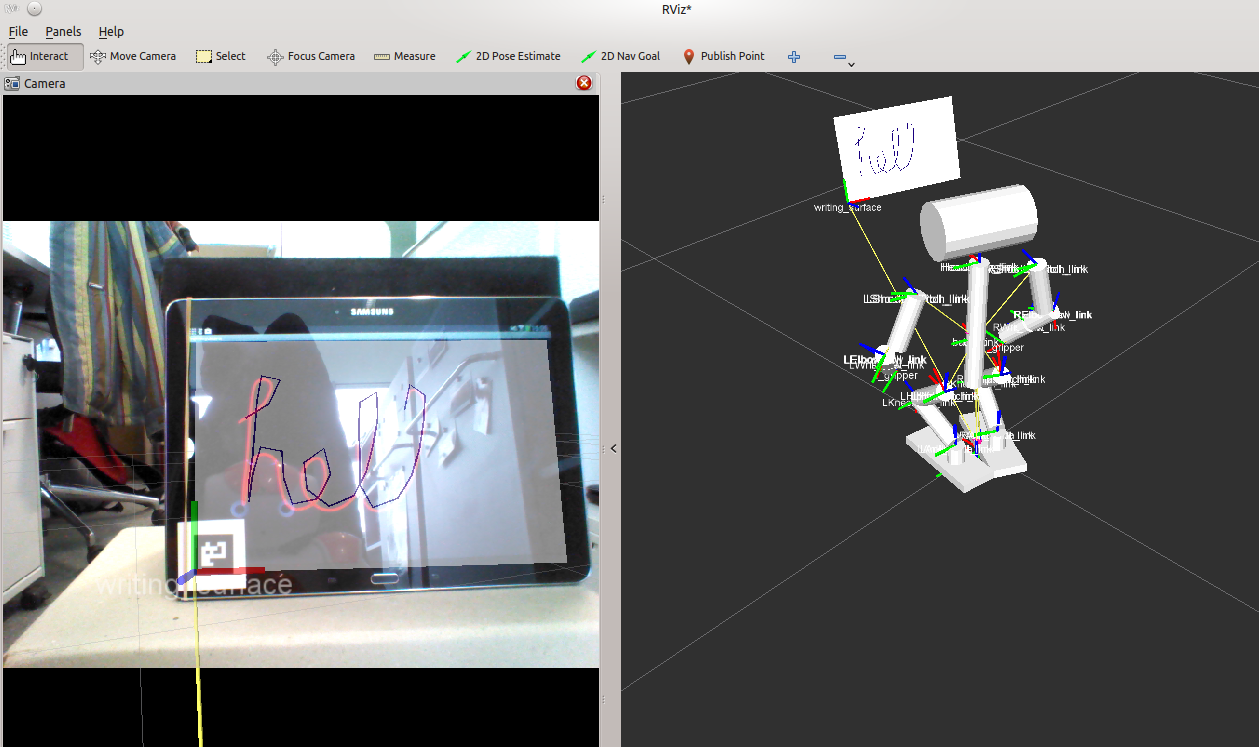
\includegraphics[width=0.9\columnwidth]{figures/chilitagDetection_cameraOverlay.png}
    \caption{\label{fig:tabletDetection}Detection of the tablet using a fiducial
    marker to represent the origin of the writing surface frame, visualised in RViz. The robot's
    camera image is on the left, with the text trajectory overlay visible.}

\end{figure}


\subsection{Integration into a Teachable Robotic Agent}

The fusion of the embodied handwriting agent developed with the handwriting
learning algorithm presented in Section \ref{sec:learningAlgorithm} involves the
integration of three components: the robot, the tablet, and a central controller
(Figure~\ref{fig:archi}). The robot and Android tablet application present the
writing process/result to the user, as explained in the previous section.
The tablet application has been extended to act as the primary medium for
capturing participant input, and submits the user's demonstrations when they are
satisfied with their writing. 

The user demonstrations are received by the
interaction controller running on a desktop computer. It is responsible for
getting the {\sc nao} to prompt and respond appropriately to feedback received using
a finite state machine to manage the interaction stage and various system
inputs. In the context of learning handwriting, an additional input to the system 
is a word from which the letters are to be learned, which is detected by a fiducial 
marker on the card displaying the word.
The controller provides inputs to the learning algorithm including the word to learn
and the user demonstrations, by inferring the letter which the demonstrations are 
intended for based on their position on the tablet. The output shapes from the 
learning algorithm are sent by the controller to the devices which write them.

The source code for the teachable robotic handwriting partner has been made 
%available at \url{https://github.com/chili-epfl/cowriter_letter_learning}.
available at \url{[anonymized]}.


%Feedback from the user is passed to the controller with the location on the
%tablet that it occurred at, and the task of interpreting the shape which the
%feedback was intended for is left to the controller as it is aware of the
%location of published shapes. The appropriate response in terms of the learning
%algorithm is then taken for the respective shape. 

%make line colours not colour dependent
\begin{figure}[ht]
\centering

\resizebox{0.9\linewidth}{!}{%

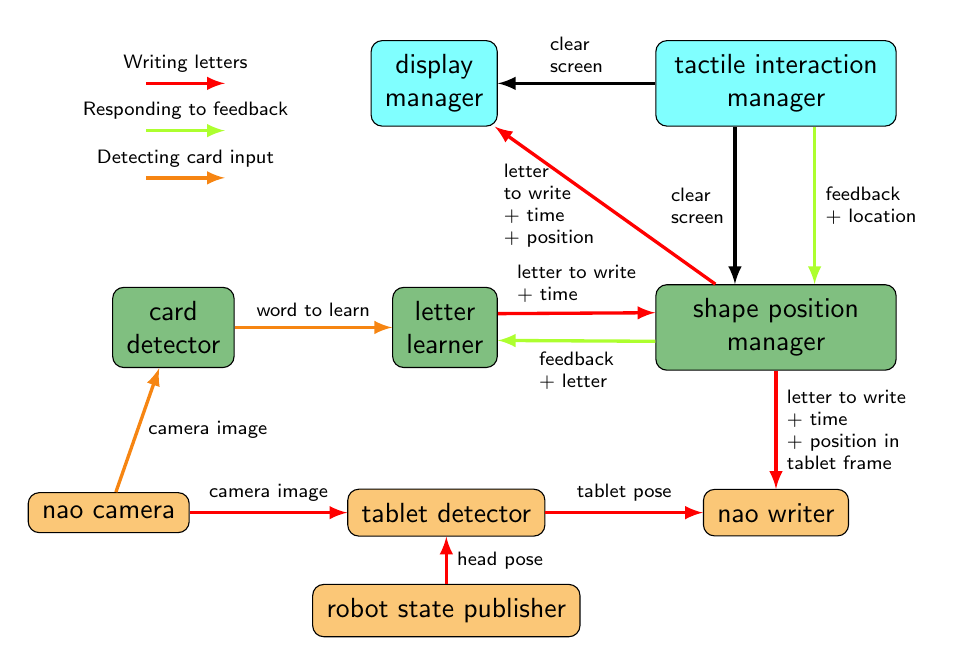
\begin{tikzpicture}[
    >=latex,
    node distance=2cm,
    every edge/.style={draw, very thick},
    redarrow/.style={fill=Red, draw=Red},
    greenarrow/.style={fill=GreenYellow, draw=GreenYellow},
    yellowarrow/.style={fill=BurntOrange, draw=BurntOrange},
    cmpt/.style={draw, align=center, rounded corners, inner sep=5pt, font=\sf, fill=black!20},
    label/.style={midway, align=left, font=\scriptsize\sf, fill=white, above,opacity=0,text opacity=1}]

    \node at (0,0)[cmpt, fill=Cyan!50, text width=2.7cm] (tactile) {tactile interaction \\ manager};
    \node[cmpt, fill=Cyan!50, left=of tactile] (display) {display \\ manager};
  
    \node [cmpt, fill=Green!50, below=of tactile, text width=2.7cm] (shape) {shape position \\ manager};
    \node [cmpt, fill=Green!50, left=of shape] (learner) {letter \\ learner};
    \node [cmpt, fill=Green!50, left=of learner] (card) {card \\ detector};

    \node [cmpt, fill=YellowOrange!50, below=1.5cm of shape] (writer) {nao writer};
    \node [cmpt, fill=YellowOrange!50, left=of writer] (tablet) {tablet detector};
    \node [cmpt, fill=YellowOrange!50, left=of tablet] (camera) {nao camera};
    \node [cmpt, fill=YellowOrange!50, below=0.6cm of tablet] (pose) {robot state publisher};

    %%% Relations between components
    \path (tactile) edge [->] node[label] {clear \\ screen} (display);

    \path ($(shape.north west)!0.33!(shape.north east)$) edge [<-] node[label,left] {clear \\ screen} ($(tactile.south west)!0.33!(tactile.south east)$);
    \path ($(shape.north west)!0.66!(shape.north east)$) edge [<-, greenarrow] node[label,right] {feedback \\ + location} ($(tactile.south west)!0.66!(tactile.south east)$);

    \path (shape) edge [->, redarrow] node[label, left, align=left] {letter \\to write \\ + time \\ + position} (display);
    \path (shape) edge [->,redarrow] node[label, right] {letter to write \\ + time \\ + position in\\tablet frame} (writer);

    \path ($(shape.north west)!0.66!(shape.south west)$) edge [->, greenarrow] node[label,below] {feedback \\ + letter} ($(learner.north east)!0.66!(learner.south east)$);
    \path ($(shape.north west)!0.33!(shape.south west)$) edge [<-, redarrow] node[label] {letter to write \\ + time} ($(learner.north east)!0.33!(learner.south east)$);

    \path (card) edge [->, yellowarrow] node[label] {word to learn} (learner);
    \path (camera) edge [->, yellowarrow] node[label, right] {camera image} (card);
    \path (camera) edge [->, redarrow] node[label] {camera image} (tablet);
    \path (tablet) edge [->, redarrow] node[label] {tablet pose} (writer);
    \path (pose) edge [->, redarrow] node[label, right] {head pose} (tablet);

    \path (-8, 0) edge [->, redarrow] node[label] {Writing letters} (-7, 0);
    \path (-8, -0.6) edge [->, greenarrow] node[label] {Responding to feedback} (-7, -0.6);
    \path (-8, -1.2) edge [->, yellowarrow] node[label] {Detecting card input} (-7, -1.2);
    
\end{tikzpicture}
}

\caption{Overview of the system. Components in the top row run on the tablet, 
those in the middle row on the central controller, and those in the bottom row 
on the robot.}

    \label{fig:archi}
\end{figure}



%%%%%%%%%%%%%%%%%%%%%%%%%%%%%%%%%%%%%%%%%%%%%%%%%%%%%%%%%%%%%%%%%%%%%%%%%%%%%%%%

%%%%%%%%%%%%%%%%%%%%%%%%%%%%%%%%%%%%%%%%%%%%%%%%%%%%%%%%%%%%%%%%%%%%%%%%%%%%%%%%

\section{A Tool for Social and Pedagogical Investigations} \label{sec:experiment}
\label{sec4}

In addition to constituting a technically novel system, the presented teachable
robotic agent represents a tool which may be used for investigating social and
pedagogical research questions. For example, one such question is what impact the addition of
such a teachable robotic agent would have on the outcomes of a typical
handwriting intervention. 
Preliminary studies at two schools in the Geneva area, involving over 50 children, 
have been conducted to evaluate the feasibility and technical soundness of the 
interaction system proposed as a tool for such investigations.

\subsection{Interaction Context}

%The interaction context which has been developed as a framework for addressing
%relevant research questions is 
%Participants are asked to improve the robot's
%handwriting by correcting the letters it writes on the tablet. 
Figure~\ref{fig:pilotInteraction}
illustrates an example interaction sequence between the participant and the
robot which consists of the following stages:

\begin{enumerate}

    \item The participant shows the robot one of seven different 3-letter words
        to write, are made up of 7 possible letters (`c', `e',
        `n', `o', `s', `u', `w'). Fiducial markers which are printed on the word
        cards allow them to be detected with the robot's camera. 

    \item The robot responds to the word request verbally and writes the
        letters according to the method described in Section \ref{sec:tabletSynch}. 

    \item The robot asks for feedback from the participant and they demonstrate
        how to write the letter which they feel needs to be corrected. The
        tablet may be moved into the most appropriate position for the child to
        write on it with the stylus. Only one letter may be demonstrated at a time and the
        position of the participant's demonstration on the tablet encodes the
        letter that it is a demonstration for. The participant can remove and
        repeat their letter if they are unhappy with it.
        %, or if it is in the wrong position as determined by the researcher
        %conducting the interaction
        When the participant is satisfied with the demonstration, they press a button on
        the tablet which signals that it is the robot's turn.

    \item The robot writes an adapted letter in 
        response to the participant's feedback, and the interaction iterates,
        with participants taking turns to interact with the robot if necessary.
        When the participant(s) is/are satisfied with the robot's performance on 
	all letters,
        they may use the ``test'' card and an additional word for which they will
        verbally evaluate the robot's performance. 

\end{enumerate}


\begin{figure}[thpb!]
     \begin{center}
%
        \subfigure[The user shows a card to the robot with a word to write.]{%
            \label{fig:first}
            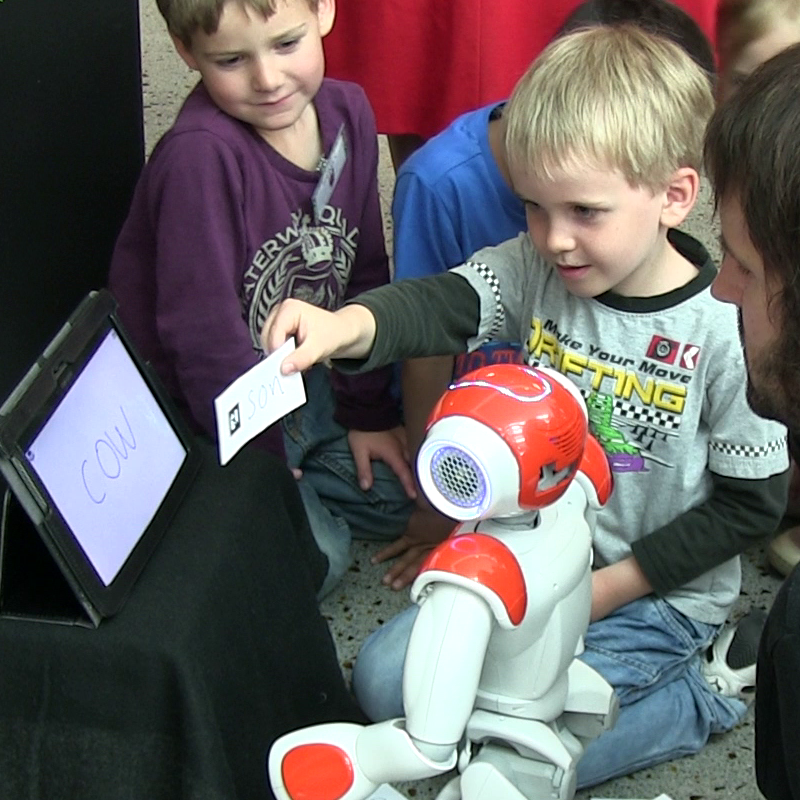
\includegraphics[width=0.2\textwidth]{figures/1card.png}
        }~
        \subfigure[The robot writes the word seen on the card and asks for feedback.]{%
           \label{fig:second}
           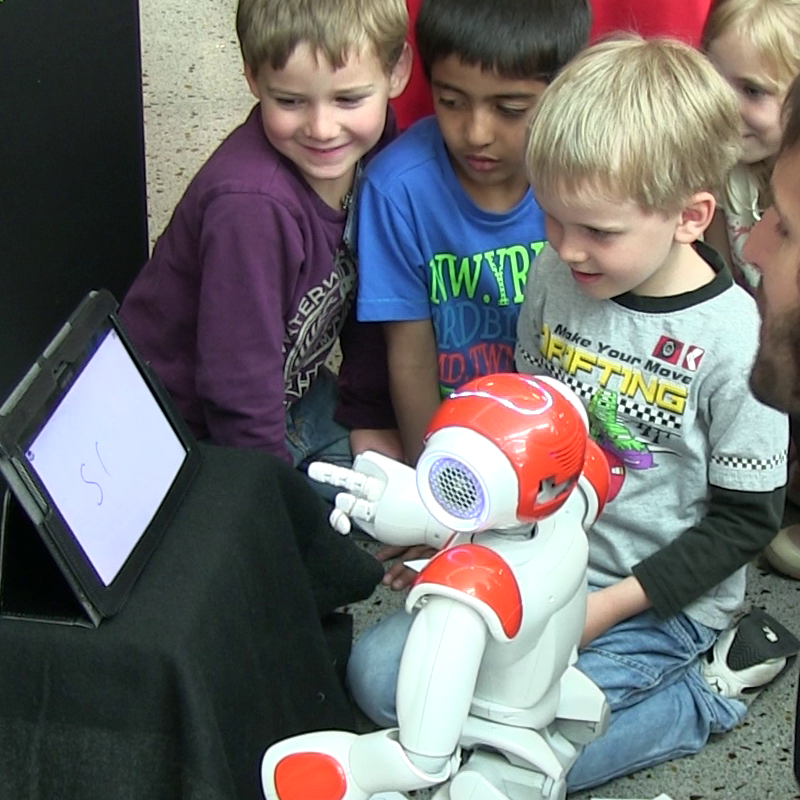
\includegraphics[width=0.2\textwidth]{figures/2word.png}
        }\\ %  ------- End of the first row ----------------------%
        \subfigure[The user provides feedback on the letters written via demonstration.]{%
            \label{fig:third}
            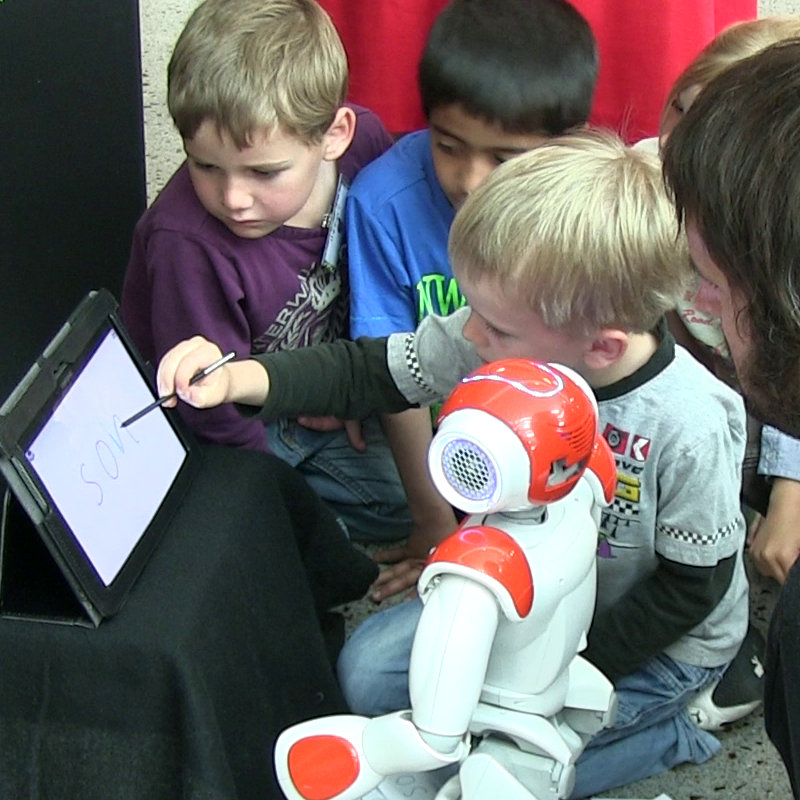
\includegraphics[width=0.2\textwidth]{figures/4correct.png}
        }~
        \subfigure[The robot responds to the feedback, until the user is satisfied.]{%
            \label{fig:fourth}
            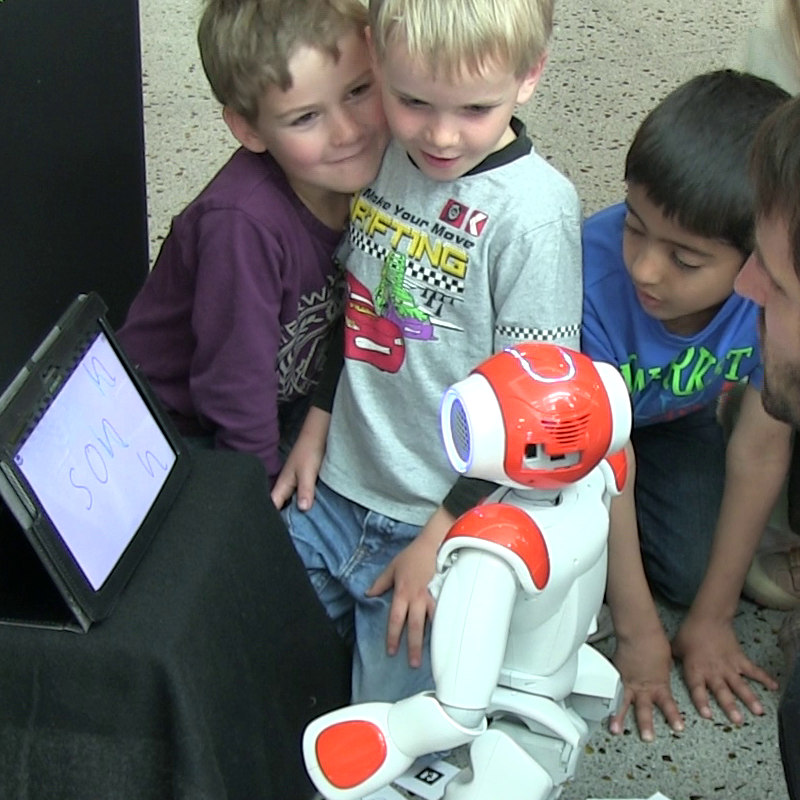
\includegraphics[width=0.2\textwidth]{figures/5iterateAsk.png}
        }%
%
    \end{center}
    \caption{%
        A user engaging with the robot in the \emph{learning by teaching}
    interaction, using demonstrations as feedback.}%

   \label{fig:pilotInteraction}
\end{figure}

\subsection{Outcomes of Preliminary Study 1}


A pilot study at the first school consisted of four groups of
approximately 8 english-speaking children each, aged 6-7 years. The children
interacted with the system for a total of 65 minutes, with the robot writing 96
letters. 49 of these letters were in response to demonstrations from the children 
and the remaining were from when new words were requested. 

As a result of the pilot study, two key observations were acted on. The first
was that children appeared to have a difficult time providing demonstrations to
the robot in the same place as previously-written letters. At the time, the
system required the children to write on top of a letter of the same type as the
one which they were demonstrating, and the children seemed to find this
counter-intuitive and would occasionally just trace the robot's letter as it
appeared. As such, the technical components of the system were extended to allow
the children the opportunity to write around previously-written letters instead
of on top. 

The second key point which came from the pilot study was that children were
observed giving advice to the child designated as the letter demonstrator,
potentially giving rise to a higher level paradigm of learning by
\emph{teaching to teach}. As a consequence of this observation, the study which
followed at the second school was designed to further observe the effect of the
number of children interacting with the robot.

\subsection{Outcomes of Preliminary Study 2}
The study at the second school involved 21 french-speaking students aged 7-8 years. 7 children
interacted with the robot individually and 7 sessions included the remaining
14 students interacting with the robot in pairs.
Initial parameters were drawn from a range purposely chosen to generate shapes 
for letters 'e' and 's' which would elicit correction. For the other letters, 
parameters were fixed, generating shapes which some groups still chose to correct 
(e.g. 13/14 for 'n' and 2/14 for 'c'). The duration of the sessions
was between 8 and 15 minutes, with an average of 11.4 minutes (SD = 2.3). 

%The following conclusions were successfully drawn about the system as a result
%of the study at the second school.

It has been concluded following the second study that the system has 
been validated as a technically sound autonomous interaction. 
The interaction setup including the teachable
robotic agent withstood the interaction which lasted for a total of 160 minutes. 
During this time the robot wrote 335 letters, 152 of which in response to
demonstrations received from the 21 children. Technical 
intervention was only required for the three instances that the robot fell 
later in the day. Otherwise, the technical components of the system operated 
autonomously and as expected over the sessions.

Furthermore, no child indicated that they did not believe that the robot was writing
by itself. There were, at times, 
    questions about the robot's writing method at the beginning of the interaction,
    but when advised that the robot ``tells the tablet what it wants to write,''
    this was accepted by the children. 
%     To allow the children an opportunity to
%     express doubt in the robot's ability to write without explicitly asking them if
%     the robot was pretending, the children were asked if they believed that the
%     robot would be able to write its name, \emph{{\sc nao}} which had not previously been
%     demonstrated. It was reasoned that this would prompt the children to question
%     the point of the robot actually \emph{writing} if they had any suspicion that
%     the robot was pretending, but this was never the case. 
    On the rare occasion that the
    robot's writing was not correctly synchronised with the tablet, this did
    not appear to influence the children's impression. 
    If older children participate in the interaction study --
    which may be likely as children with lasting handwriting difficulties are included
    as participants -- it may become more important to invest time into the
    believability of the robot's writing scheme. However, for 6-8 year olds the
    proposed setup appears sufficient.

Regarding the engagement of the children in teaching the robot, 
    an average of 10.9 demonstration letters (SD = 4.4) were
    provided to the robot for each session during the interaction.
    In 9 out of the 14 sessions (64\%), the robot received demonstration letters
    even \emph{after} reaching the test stage of the interaction. The participants'
    teaching after the test word had been written and evaluated -- the only
    purposefully imposed external motivation -- may suggest that by that time
    the participants had become intrinsically motivated to engage in the
    interaction.

%     \textbf{All children believed that the robot was learning and that
%         they were the ones teaching it.} This was concluded from the responses
%         when the children were asked directly. This is in contrast to a prior
%         feasibility study for a version of the interaction which only allowed
%         for touch-based feedback, not user demonstrations, in which three of the
%         seven adult participants did not feel that it was their input which
%         helped the robot improve.

    %, and also their reaction to the ``test word'' written by the robot at the end of the interaction. In X\% of cases, the child concluded that the robot had `passed' the test, or congratulated it in some way.



%%%%%%%%%%%%%%%%%%%%%%%%%%%%%%%%%%%%%%%%%%%%%%%%%%%%%%%%%%%%%%%%%%%%%%%%%%%%%%%%
\section{Towards Long-term Studies}\label{sec:futureWork}
%How to break this section up?

A conclusion drawn in a systematic review of handwriting intervention studies~\cite{Hoy2011} 
is that any of the studies considered which involved 
fewer than two practice sessions per week and fewer than a total of 20 practice 
sessions, including homework, were not found to demonstrate effective results. This 
highlights the necessity to engage students in an interaction which will be sustainable
 over the long-term if 
we want to address research questions which involve the measurement of learning gains. 
Several challenges are raised in developing such long-term capabilities for the system,
 from both technical and sociological points of view. %not sure this makes sense

In terms of the interaction experience, the current experimental setting, while
technically autonomous, can not robustly recover from situations outside of the
nominal protocol presented in Section~\ref{sec4}, and consequently still
requires the presence of an experimenter. The interaction finite state machine would
require extension in non-trivial ways to allow for long, fully autonomous
interactions with children.

In the current system, the robot can ask questions and prompt participants, but it 
cannot engage in discussions with the participants. It is clear that work is necessary 
to develop the conversational agent in the interaction so that the presence of an 
experimenter is not required for a captivating and continuing engagement. While there is the 
possiblity to focus the interaction design on group-based interaction with the robot 
in order to alleviate the necessity of a conversational agent, there is reason to 
believe that constructing such a social interaction is not a trivial task. Anecdotes 
from the preliminary studies have shown that some children may criticise another's 
demonstrations to the robot, which may or may not be as damaging to a child's 
self-efficacy as when they are criticised in a typical educational context. In addition,
on occassions where a pair of children came to teach the robot different styles of a 
particular letter, they did not discuss with each other their different writing styles 
and the effect on the teaching efficiency. This may suggest that a constructed social context in 
which verbalising opinions about differences is encouraged may be necessary to get children 
to cooperate in teaching the robot in a group setting.  
%- "Would have problems with the 'n'" - (8) projecting human learning characteristics.
%- awkward silence, speaking over the top of the robot to talk to experimenter....
%- Children saying the other was bad... (3, 9).
%- When one child wrote u differently to the other, they didn't discuss :(

How the children's perception of the robot as a learning agent may change over the 
long-term remains to be seen. On one occasion during the preliminary studies, a 
child's response to whether or not the {\sc nao} could write its own name included that it 
may have problems with the `n', as the child had been correcting the robot on this 
letter. This suggests that users may project human-like learning features, such as 
forgetfulness, onto the robot, whether or not they are technically present.
This may need to be capitalised on when considering how to 
extend the interaction for long time frames, as the present system -- with a learning rate 
such that progress is evident to the user -- will cause convergence for a letter within a 
few iterations.

In the scope of open technical questions for enabling long-term interaction, it remains to be seen how shape models
for letters might be generated which capture the full range of mistakes typical
of children learning handwriting. This includes extending the current system capable of
incorporating internal proportion and global deformation errors to one which can
also generate missing subparts of the letter, or write letters backwards, for example. 
While it is expected that incorporating a
database of letters drawn by children into the shape modeling process would
facilitate this, the current system has conceptual -- a PCA-only approach can not
generate or learn a different shape topology -- and technical -- no support is currently implemented for
multi-stroke shapes -- limitations which would need to be overcome.

If the system is extended to allow for a wider range of mistakes, a further 
topic for exploration then is how the handwriting error
generation of the system may be abstracted to a higher level of control so that
a teacher may configure it to work with a child on a particular type of
mistakes based on the child's performance. Where would the balance lie between
developing autonomous capabilities for the system to determine the child's
difficulties and empowering the teaching staff to decide for themselves
instead? 

With some of these challenges addressed, further steps can be made towards 
answering the overarching question of what impact the 
addition of such a teachable robotic agent would have on handwriting interventions, including the effect on the 
participants' self-esteem, motivation, and learning gains. % does it impact the
%motivation of the participants, their self-esteem, and/or the learning gains
%that they experience? We are currently considering running a long-term study
%that would provide better evidences to answer these questions.


%In addition to the conclusions which 
%Anecdotes which raise questions:
% Another said "programmed to write badly" (4)
% Child saying the other child's was good (5). Child saying the robot was better than him (9).

%- so many of them wanted to write the whole word.. robot says "show me a word" and maybe misleading
%- not seeming to notice small changes (12) but maybe from experimenter
%

%- child walking around
%- word very close to robot's camera
%
%Evidence of engagement:
%- work and/or play
%- once word was good were thinking for a long time about how to improve (8)
%- child `helping' other.. grabbing the pen
%- children trying to cheat the system (10)
%- excitement at stop and test cards - new letters? diff font
%- teaching cursive. group 7 excited to do this even after test finished.
%- unnecessary (unsent) demo from child 11 after it was acceptable but not perfect


\addtolength{\textheight}{-.5cm}   % This command serves to balance the column lengths
                                  % on the last page of the document manually. It shortens
                                  % the textheight of the last page by a suitable amount.
                                  % This command does not take effect until the next page
                                  % so it should come on the page before the last. Make
                                  % sure that you do not shorten the textheight too much.

\section{Impact and Conclusion}\label{sec:conclusions}

We believe that this article introduces three noteworthy contributions: an innovative
application of data processing and artificial intelligence for the
learning of hand-written letters suitable for educative purposes; a robotic
system which has been experimentally shown to provide convincing scaffolding for
complex human-robot interactions (teacher-learner social interactions, learning by
demonstration, simulated robotic fine motor skills); and an initial experimental investigation of what appears to be a
new role for robots in education.

Specifically, the technical challenges involved in developing a teachable
robotic agent in the context of handwriting which have been addressed in this
work include:

\begin{itemize}

    \item developing capabilities for a robot with limited fine motor
        capabilities, in particular the {\sc nao} robot, to engage in the act of handwriting in a
        way which is believable for interacting with children. This is
        accomplished by leveraging simulated handwriting with a synchronised
        tablet communicating via ROS;

    \item developing an algorithm capable of incorporating user feedback and
        demonstrations in order to adapt artificially generated handwriting quality so as
        to simulate a teachable agent, which has been implemented by maintaining
        a learning algorithm in the parameter space of the PCA-based shape models and
        converging towards the parameters of user demonstrations; and

    \item integrating the system into a working interaction suitable for
        engaging children in the learning by teaching paradigm, accomplished by
        fusing the robotic drawing capabilities and the learning algorithm for
        handwritten letters established with a central controller which manages
        the flow of the interaction, turn taking and integration of the connected 
	devices.

\end{itemize}


However, we believe that the strongest impact of this work is for the human-robot
interaction community and relates to the very \emph{nature} of the interaction
fostered by this research. The work presented here investigates a particular
role for a robot in the education of handwriting: not only is the robot actively
performing the activity by drawing letters, but it does so in a way that engages
the child in a very specific social role. The child is the teacher in this relationship and the robot is
the learner: the child must engage in a (meta-) cognitive relationship with the robot
to try to understand why the robot fails and how to help it best.  Here, the
robot is more than just an activity facilitator or orchestrator -- its physical presence
and embodiment induce agency and anthropomorphising, and cognitively engage the
child into the learning activity, which we predict will lead to higher learning
efficacy.

Also notable, the robot is not used in the usual context of robotics or computer
education, but instead in an activity -- handwriting -- which requires fine
physical skills. In such activities, the embodied nature of the robot is appropriate as in interventions where motor mimicry is elicited \cite{Berninger1997} the arm motion for instance is, \emph{by
itself}, part of the teaching. Furthermore, when facing a child with school 
difficulties, robots can play the role of a na\"ive learner which neither adults 
nor peers -- because of the social effects it would induce -- can convincingly 
play. Along these lines, we hope to see more research
on non-STEM educational applications of robotics.

% Beyond handwriting, we believe that this work provides a novel perspective on
% the role for robots in the field of education. \emph{Learning by teaching} is a
% powerful paradigm because of not only its pedagogical efficacy, but its
% potential to positively impact the child's motivation and self-esteem. We hope that 
% this article shows that this is a very relevant context of use for robots. Indeed,
% when facing a child with school difficulties, robots can play the role of a na\"ive 
% learner which neither adults nor peers -- because of the social effects it would 
% induce -- can convincingly play.

The strong social impact of early educational problems makes continued research in this field
an undoubtedly meaningful challenge for robotics and human-robot interaction.

%%%%%%%%%%%%%%%%%%%%%%%%%%%%%%%%%%%%%%%%%%%%%%%%%%%%%%%%%%%%%%%%%%%%%%%%%%%%%%%%
% Anonymized for double-blind review
%\section*{Acknowledgments}
%
%This research was supported by the Swiss National Science Foundation through the
%National Centre of Competence in Research Robotics.

%%%%%%%%%%%%%%%%%%%%%%%%%%%%%%%%%%%%%%%%%%%%%%%%%%%%%%%%%%%%%%%%%%%%%%%%%%%%%%%%

%\begin{thebibliography}
\bibliographystyle{abbrv}
\bibliography{library}

%\end{thebibliography}

\end{document}
